
It could be interesting to find out what the escape velocity of the Sun is. We
can find this value experimentally by simulating the Sun-Earth system with
various initial velocities for the Earth. By trial and error, we concluded that
the escape velocity lies in the range $v = 8.85 - 8.89$ AU/yr. Figure
\refig{escapevel} shows Earth leaving the system with $v = 8.89$ AU/yr.
%
\begin{figure}[htpb]
	\centering
	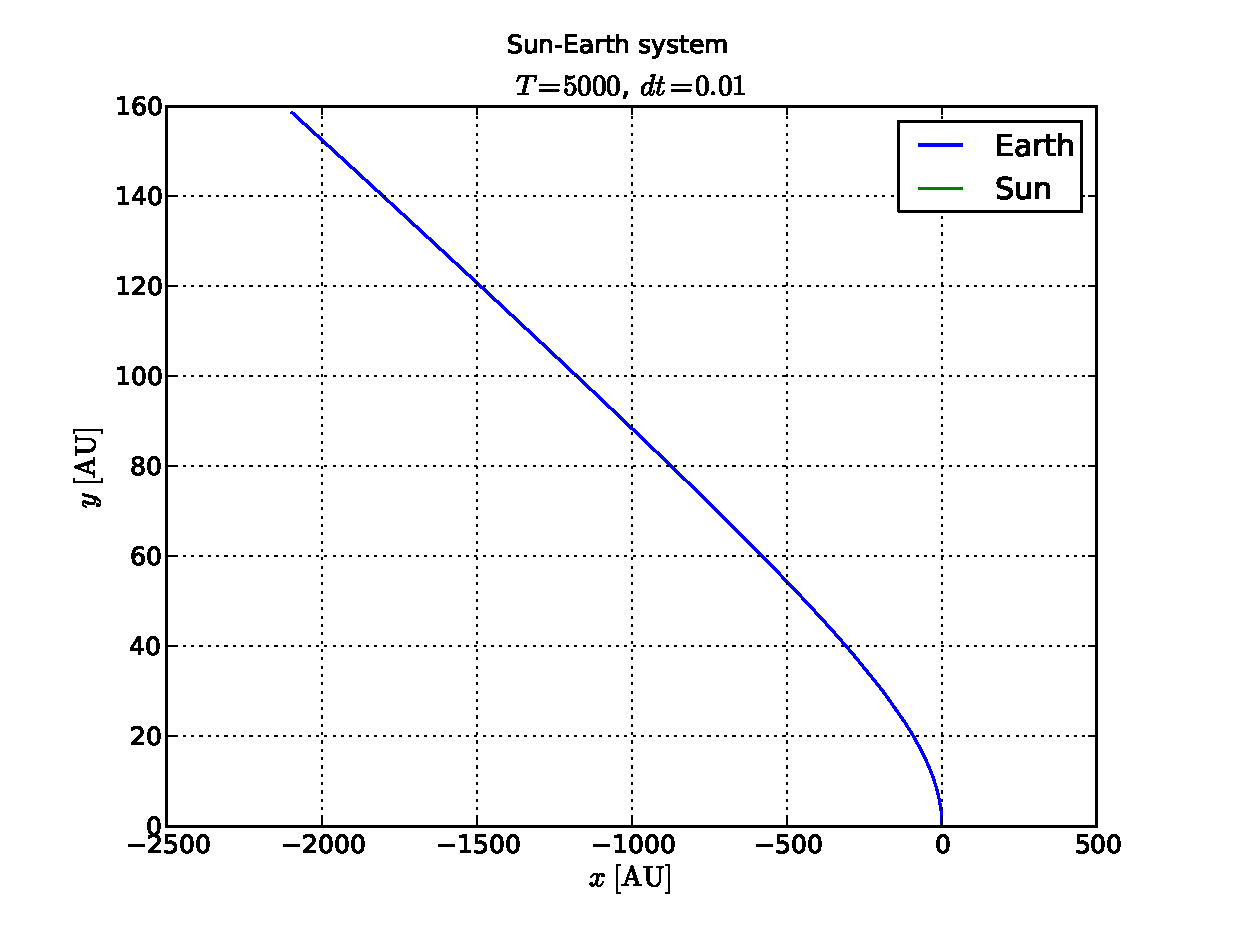
\includegraphics[width=0.8\textwidth]{figures/sun_earth_T5000_dt1e-2}
	\caption{Earth leaving the system at a velocity $v = 8.89$ AU/yr higher
		than the escape	velocity.}
	\label{fig:escapevel}
\end{figure}
%
We see that the Earth starts on a very eccentric elliptical orbit, but has a
velocity that is too high to make the bend, so it escapes on an asymptotic
path, giving it a hyperbolic trajectory instead.

We can find an exact answer to the Sun's escape velocity by using the fact that
Earth is free of the gravitational attraction from the Sun when
\begin{equation}
	E = E_k + E_p = 0
	\label{eq:Eequal0}
\end{equation}
where $E_k$ is the Earth's kinetic energy, and $E_p$ is the potential energy. We
need to find the velocity $v$ that makes \refeq{Eequal0} true.
%
\begin{align*}
	\frac{1}{2}M_{\text{Earth}}v^2 &- G \frac{M_{\odot} M_{\text{Earth}}}{r}
	= 0 \\
	\frac{1}{2}M_{\text{Earth}}v^2 &= G \frac{M_{\odot} M_{\text{Earth}}}{r} \\
	v^2 &= 2\frac{GM_{\odot}}{r} \\
	v &= 2\sqrt{2}\pi \approx 8.886 \ \text{AU/yr}
\end{align*}
%
where we have used that $GM_{\odot} = 4\pi^2$, $r = 1$ AU. From this, we see
that the experimental result we found from our simulation is quite accurate.
